\chapter{Résultats de simulation et analyse du modèle à état discret (\textit{2 pages max})}
\label{ch:simu}

Afin de valider les constats émis au chapitre \ref{ch:modele_discret}, cette partie se propose d'effectuer des simulations numériques afin d'étudier la stabilité des différents points d'équilibre.

Pour ce faire, ce chapitre se consacre à l'analyse de bifurcation, comme déjà utilisée dans \cite{ChaosControl}. Le code fourni en complément du rapport est fortement basé sur le tutoriel d'analyse de bifurcation pour Python présenté en \cite{bifurc} avec l'exemple de l'équation logistique.

\begin{figure}
    \label{fig:bifurc 1}
    \begin{center}
		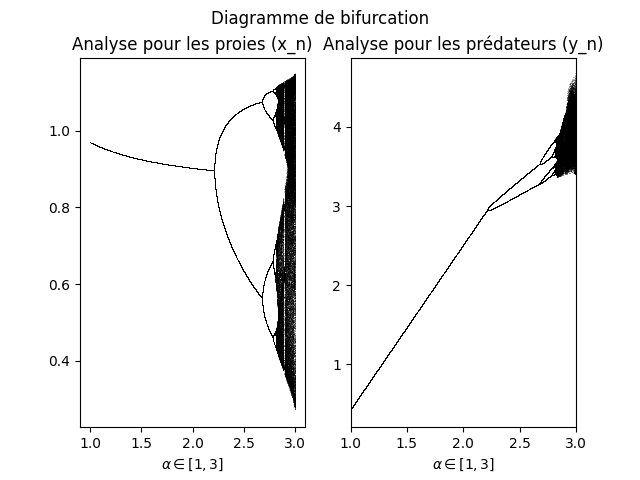
\includegraphics[width=17cm]{figures/Bifurcation_1.png}
	\end{center}
	\caption{Analyse de bifurcation pour les paramètres $\alpha \in [1, 3]$; $\beta = 0.08$; $\gamma = \alpha$; $\rho = 0.08$; $\sigma = \frac{1}{10}\alpha$ et $\nu = 0.04$ avec les conditions initiales $x_0 = 1.1$ et $y_0 = 1$}
\end{figure}


Le Chapitre \ref{ch:simu} porte sur la \textit{présentation des résultats de simulation} (ne pas oublier de préciser les valeurs numériques des paramètres considérés) et l’\textit{analyse des résultats de simulation obtenus en utilisant le modèle à état discret}.
Ce chapitre permettra de valider en simulation le modèle à état continu, complétant les réponses aux questions I.1, I.2 et I.3 du sujet.
